% !TeX root = ../main.tex
% Add the above to each chapter to make compiling the PDF easier in some editors.

\chapter{Probability}

\section{Random Walks}

In this section, we study random walks on undirected weighted graphs $G = (\sV, \sE, \vw)$ with self-loops. A \emph{random walk}\index{random walk} visits a random sequence of vertices $v_1, v_2, \dots$, where \begin{align}
    \Pr{v_{t+1} = v \mid v_t = u} = \frac{\vw(\{v, u\})}{\vd(u)}
\end{align} and $\vd(u)$ is the weighted degree of vertex $u$, as we have defined previously.

\begin{rmk}
The random walks considered here satisfy the \emph{Markov property}\index{Markov property}, that is, \begin{align}
    (v_{t+1} = v) \perp (v_1 = u_1), \dots, (v_{t-1} = u_{t-1}) \mid (v_t = u_t).\safefootnote{So you can think of these random walks as Markov chains.}
\end{align} Moreover, we restrict our attention to time-homogeneous random walks, that is, the transition probabilities remain constant over time.
\end{rmk}

We can therefore model the update of a single round using the linear map $\mW \in \R^{|\sV|\times|\sV|}$ (called \emph{transition matrix}\index{transition matrix}), \begin{align}
    \mW \defeq \begin{bmatrix}
    \frac{\vw(\{1,1\})}{\vd(1)} & \cdots & \frac{\vw(\{n, 1\})}{\vd(n)} \\
    \vdots & \ddots & \vdots \\
    \frac{\vw(\{1,n\})}{\vd(1)} & \cdots & \frac{\vw(\{n, n\})}{\vd(n)} \\
    \end{bmatrix} = \mA\inv{\mD}.
\end{align}

A probability distribution over vertices is a vector $\vp \in \R^{|\sV|}$ such that $\trans{\vOne}\vp = 1$ and $\vp \geq \vZero$. If our initial distribution is $\vp_0$, we have, \begin{align}
    \vp_t = \mW^t\vp_0.
\end{align}

\begin{defn}[Stationary distribution] A distribution $\vpi \in \R^{|\sV|}$ is \emph{stationary}\index{stationary distribution} iff $\vpi = \mW\vpi$.
\end{defn}
\begin{lem}
Every graph has the stationary distribution $\vpi \defeq \frac{\vd}{\trans{\vOne}\vd}$.
\end{lem}\begin{proof} First, $\pi$ is a distribution as, \begin{align*}
    \trans{\vOne}\vpi = \frac{\trans{\vOne}\vd}{\trans{\vOne}\vd}
\end{align*} and clearly $\vpi \geq \vZero$. We have, \begin{align*}
    \mW\vpi = \frac{1}{\trans{\vOne}\vd}\mA\inv{\mD}\vd = \frac{1}{\trans{\vOne}\vd}\mA\vOne = \frac{\vd}{\trans{\vOne}\vd} = \vpi. &\qedhere
\end{align*}
\end{proof}
\begin{rmk}
When the graph is connected, this is the unique stationary distribution.\footnote{In the context of Markov chains, irreducibility is sufficient for a unique stationary condition and equivalent to the transition graph being connected.}
\end{rmk}

\subsection{Lazy Random Walk}

\begin{marginfigure}
\centering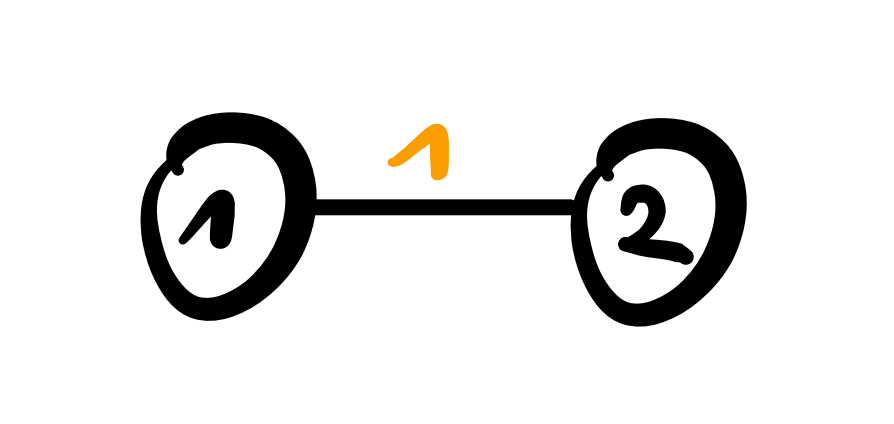
\includegraphics[width=3cm]{notes/figures/not_aperiodic.png}
\caption{Consider the initial distribution $\vp_0(1) = 1, \vp_0(2) = 0$. Clearly, the random walk will forever oscillate between the two states.}\label{fig:not_aperiodic}
\end{marginfigure}

We would also like to have that we converge to this stationary distribution regardless of the initial distribution $\vp_0$, but this is not true for general graphs, as is shown in \cref{fig:not_aperiodic}. A sufficient condition for convergence to the stationary distribution is, however, that all vertices have self-loops.\footnote{It is easy to check that this ensures that the Markov chain is aperiodic, which together with irreducibility implies convergence to the unique stationary distribution.}

Given the random walk $\mW$, the associated \emph{lazy random walk}\index{lazy random walk} is given by, \begin{align*}
    \Tilde{\mW} \defeq \frac{1}{2}\mI + \frac{1}{2}\mW,
\end{align*} that is, we add self-loops to each vertex with weight $\nicefrac{1}{2}$ and halve all other weights. Observe that this does not change the stationary distribution of the random walk. This ensures that the following holds.

\begin{thm}[Convergence of lazy random walk]\label{thm:convergence_of_lazy_random_walk}
For a connected graph, the lazy random walk converges to its unique stationary distribution irrespectively of the initial distribution $\vp_0$, \begin{align}
    \lim_{t\to\infty} \Tilde{\mW}^t\vp_0 = \Tilde{\vpi} = \vpi.
\end{align}
\end{thm}

To prove this theorem, let us first understand the transition matrix in terms of the graph Laplacian.

\begin{lem}
When $\nu_1, \dots, \nu_n$ are the eigenvalues and $\vpsi_1, \dots, \vpsi_n$ the corresponding eigenvectors of the normalized Laplacian matrix $\mN$, then $\Tilde{\mW}$ has eigenvalues $1 - \nicefrac{\nu_i}{2}$ and (not necessarily orthogonal) eigenvectors $\mD^{\frac{1}{2}}\vpsi_i$.
\end{lem}\begin{proof} Let us first express the transition matrix of the original random walk in terms of the normalized graph Laplacian, \begin{align}
    \mW = \mA\inv{\mD} &= \mD^{\frac{1}{2}}(\mD^{-\frac{1}{2}}\mA\mD^{-\frac{1}{2}})\mD^{-\frac{1}{2}} \nonumber\\
    &= \mI + \mD^{\frac{1}{2}}\underbrace{(\mD^{-\frac{1}{2}}\mA\mD^{-\frac{1}{2}} - \mI)}_{-\mN}\mD^{-\frac{1}{2}} \nonumber\\
    &= \mI - \mD^{\frac{1}{2}}\mN\mD^{-\frac{1}{2}} \\
    &= \mD^{\frac{1}{2}}(\mI - \mN)\mD^{-\frac{1}{2}}. \nonumber
\end{align} By \cref{lem:a7}, $\mD^{\frac{1}{2}}(\mI - \mN)\mD^{-\frac{1}{2}}$ and $\mI - \mN$ have the same eigenvalues, namely $1 - \nu_i$. We also have, \begin{align}
    \Tilde{\mW} = \frac{1}{2}\mI + \frac{1}{2}(\mI - \mD^{\frac{1}{2}}\mN\mD^{-\frac{1}{2}}) = \mI - \frac{1}{2}\mD^{\frac{1}{2}}\mN\mD^{-\frac{1}{2}},
\end{align} implying that the eigenvectors of $\Tilde{\mW}$ are $1 - \nicefrac{\nu_i}{2}$. Finally, we have, \begin{align*}
    \Tilde{\mW}\mD^{\frac{1}{2}}\vpsi_i &= (\mI - \frac{1}{2}\mD^{\frac{1}{2}}\mN\mD^{-\frac{1}{2}})\mD^{\frac{1}{2}}\vpsi_i \\
    &= \mD^{\frac{1}{2}}\vpsi_i - \frac{1}{2}\mD^{\frac{1}{2}}\mN\vpsi_i \\
    &= \mD^{\frac{1}{2}}\vpsi_i - \frac{\nu_i}{2}\mD^{\frac{1}{2}}\vpsi_i \margintag{using that $\vpsi_i$ is an eigenvector of $\mN$ with corresponding eigenvalue $\nu_i$} \\
    &= \parentheses*{1 - \frac{\nu_i}{2}}\mD^{\frac{1}{2}}\vpsi_i. \qedhere
\end{align*}
\end{proof}

\begin{proof}[Proof of \cref{thm:convergence_of_lazy_random_walk}]
TBD
\end{proof}

\begin{thm}[Convergence rate of lazy random walk]
For any unweighted connected graph $G$, we have that at time step $t$,\footnote{We will later see that $\nu_2$ is an indicator of the ``connectedness'' of $G$.} \begin{align}
    \norm{\vp_t - \vpi}_\infty \leq e^{-\nicefrac{\nu_2 t}{2}}\sqrt{n}.
\end{align}
\end{thm}
\begin{proof}
TBD
\end{proof}

\section{Concentration}

\begin{thm}[Markov's inequality]\index{Markov's inequality}
For any random variable $X \geq 0$ and $t > 0$, \begin{align}
    \Pr{X \geq t} \leq \frac{\E{X}}{t}.
\end{align}
\end{thm}
\begin{proof} We have, \begin{align*}
    \E{X} = \int_0^\infty x f(x) \,dx \geq \int_t^\infty x f(x) \, dx \geq t \int_t^\infty f(x) \,dx = t \Pr{X \geq t},
\end{align*} where $f$ is the probability density function of $X$.
\end{proof}

\begin{thm}[Jensen's inequality]\index{Jensen's inequality}
For a random variable $X$, if $f$ is convex, then $\E{f(X)} \geq f(\E{X})$.\footnote{Proof of the finite form in \cref{thm:a8}.}
\end{thm}
\begin{marginfigure}
TBD
% \centering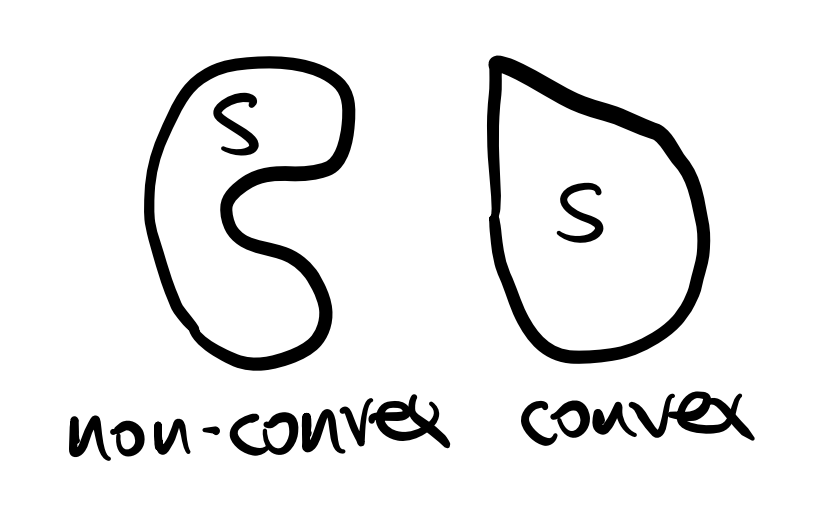
\includegraphics[width=4cm]{notes/figures/convex_set.png}
\caption{Jensen's inequality.}
\end{marginfigure}

\begin{thm}[Bernstein concentration bound]\index{Bernstein concentration bound} Given independent real-valued random variables $X_1, \dots, X_k \in \R$ such that $\E{X_i} = 0$ and $|X_i| \leq R$. Let $X \defeq \sum_i X_i$ and $\sigma^2 \defeq \Var{X} = \sum_i \E{X_i^2}$. Then, for $t > 0$, \begin{align}
    \Pr{|X| \geq t} \leq 2 \exp\parentheses*{\frac{-t^2}{2Rt + 4\sigma^2}}.
\end{align}
\end{thm}
\begin{proof}
TBD
\end{proof}

\begin{thm}[Bernstein matrix concentration bound]\index{Bernstein matrix concentration bound} Suppose $\rX_1, \dots, \rX_k \in \R^{n \times n}$ are independent symmetric matrix-valued random variables satisfying $\E{\rX_i} = \mZero$ and $\norm{\rX_i}_2 \leq R$. Let $\rX \defeq \sum_i \rX_i$ and $\sigma^2 \defeq \Var{\rX} = \sum_i \E{\rX_i^2}$. Then, for $t > 0$, \begin{align}
    \Pr{\norm{\rX}_2 \geq t} \leq 2 n \exp\parentheses*{\frac{-t^2}{2Rt + 4\sigma^2}}.
\end{align}
\end{thm}
\begin{proof}
TBD
\end{proof}

\section{Martingales}